\section{Implementation}
\label{sec:architecture}

\framework{} consists of four key components: the \textit{Packages Permission Manager}, \textit{Policy Configurator}, \textit{Resource Access Log Reporter}, and \textit{Deceiving Module}. An overview of \framework{}'s architecture is illustrated in Figure \ref{fig:method_frmwrkArch}. \framework{} accomplishes its tasks through a series of essential functions: listing installed packages and their permissions, configuring deception policies, hooking into target app processes, and generating resource access reports for manual review.

\begin{figure}[t]
    \centering
    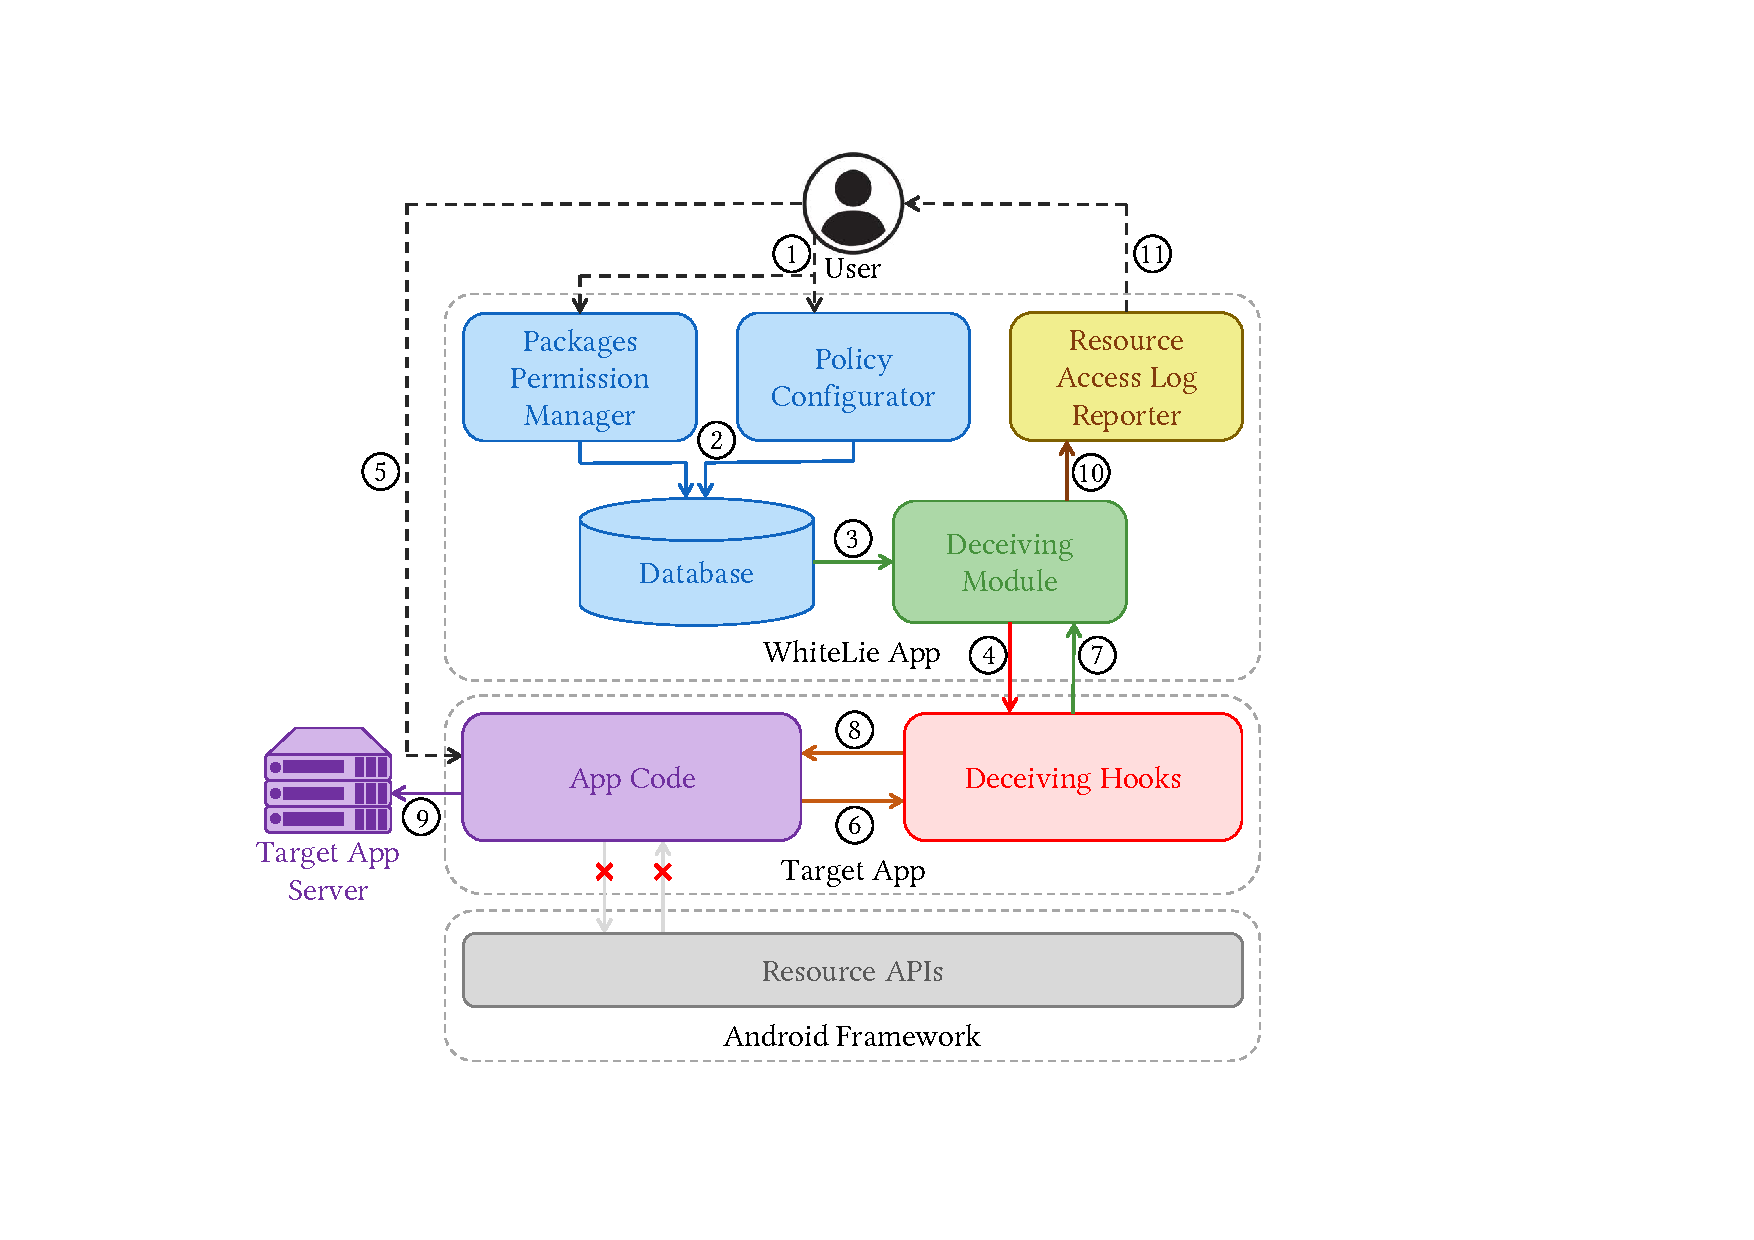
\includegraphics[width=0.65\linewidth]{Figures/Methodology/deceiver_working_architecture.pdf}
    \caption{\framework{} architecture.}
    \label{fig:method_frmwrkArch}
\end{figure}

\begin{figure}[t]
    \centering
    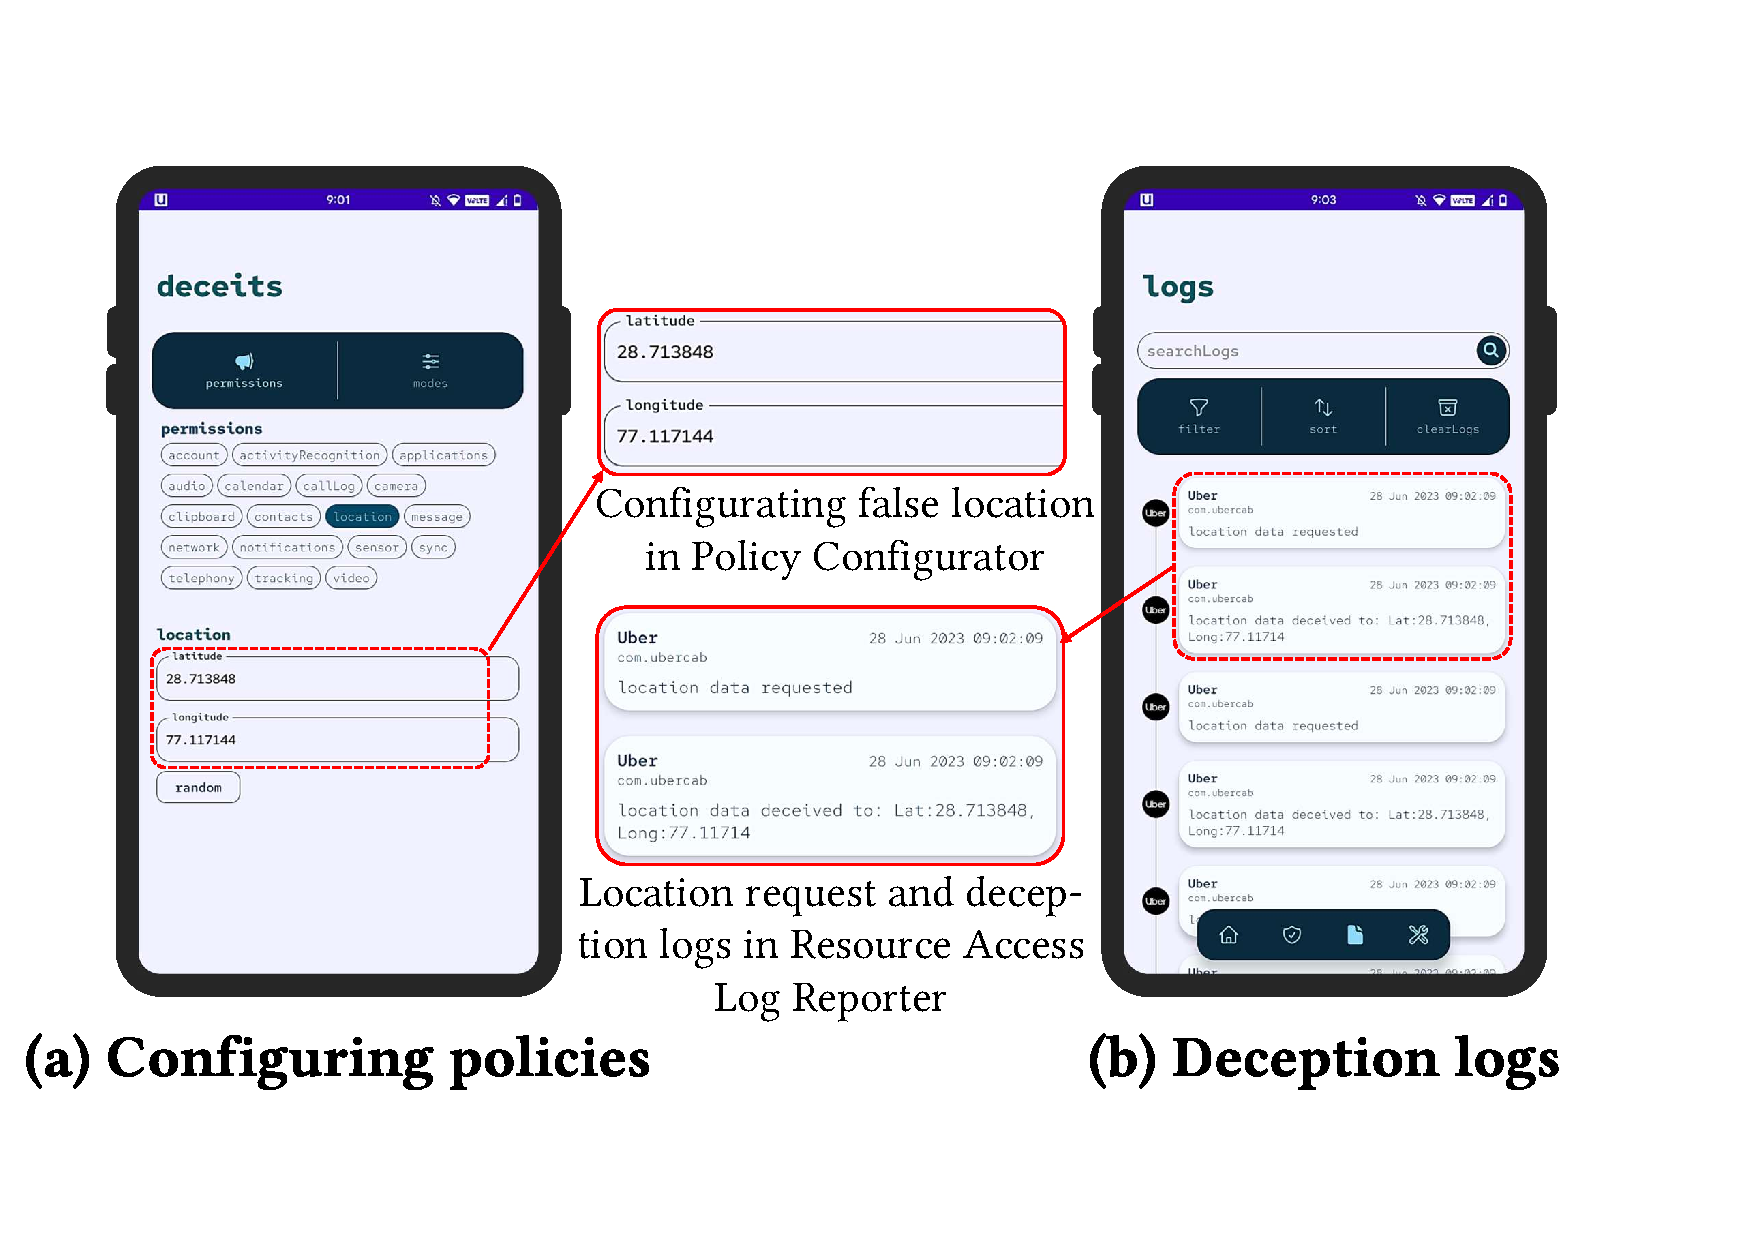
\includegraphics[width=0.75\linewidth]{Figures/Case Studies/whitelie_screenshots.pdf}
    \caption{Screenshots of \framework{} app UI while performing experiments to deceive location data for Uber.}
    \label{fig:frmwrk-ui}
\end{figure}

\circled{1}To spoof user data in target apps, the user interacts with the \textit{Package-Permission Manager} to review requested and granted permissions. \framework{} lists these using \textit{Query All Packages} permission—the only permission it requests. Installed packages are retrieved via \texttt{getInstalledApplication()} to gather app metadata. User then creates policies to spoof data for each permission. Figure\ref{fig:frmwrk-ui}a shows the \textit{Policy Configurator} UI, where a new spoofed location is defined. This customization enhances control over spoofed data, preventing privacy compromises.

\framework{} also streamlines the configuration of privacy policies by providing predefined yet configurable set of meaningful real-world values and randomly selects to efficiently safeguard user data. For example, for Contacts permission, \framework{} has a set of 100 predefined real-world contacts, that are randomly fed to the target app when requested. \circled{2}~The \textit{Package-Permission Manager} and the \textit{Policy Configurator} stores the metadata and policies defined by the user in the database. 

When the target app is launched and its process is created, the \textit{XposedBridge} class is loaded along side in the process which makes the active Xposed modules, including the \framework{} to interact with the app. \circled{3}~The \textit{Deceiving Module} of \framework{} fetches the policies defined by the user from the database and \circled{4}~accordingly installs the hooks in the target app.

\circled{5}~When the user interacts with the target app, \circled{6}~the app calls \textit{Deceiving Hooks} instead of the original sensitive Resource APIs. \circled{7}~These hooks communicate with the \textit{Deceiving Module} via \texttt{ContentProvider}, referencing stored policies to determine the appropriate spoofed data. \circled{8}~As a result, the app receives spoofed data instead of the original. \circled{9}~The app then transmits this deceived data to its server, preserving user privacy.

The installed hooks also log actions performed by the hooked app related to user data access. \circled{10}~These logs are sent to \framework{} when \textit{Deceiving Hooks} communicates with the \textit{Deceiving Module} during hooking. \circled{11}~The \textit{Resource Access Log Reporter} then shares these logs with the user for manual review. Figure \ref{fig:frmwrk-ui}b shows a screenshot of logs recorded during experiments.